\documentclass[tikz, border=0mm]{standalone}
\usepackage{ytableau}
\usetikzlibrary{calc}

\newcommand{\tikzsetnextfilename}[1]{}

\ytableausetup{boxsize=0.99em}

\begin{document}
\tikzsetnextfilename{catabolism}
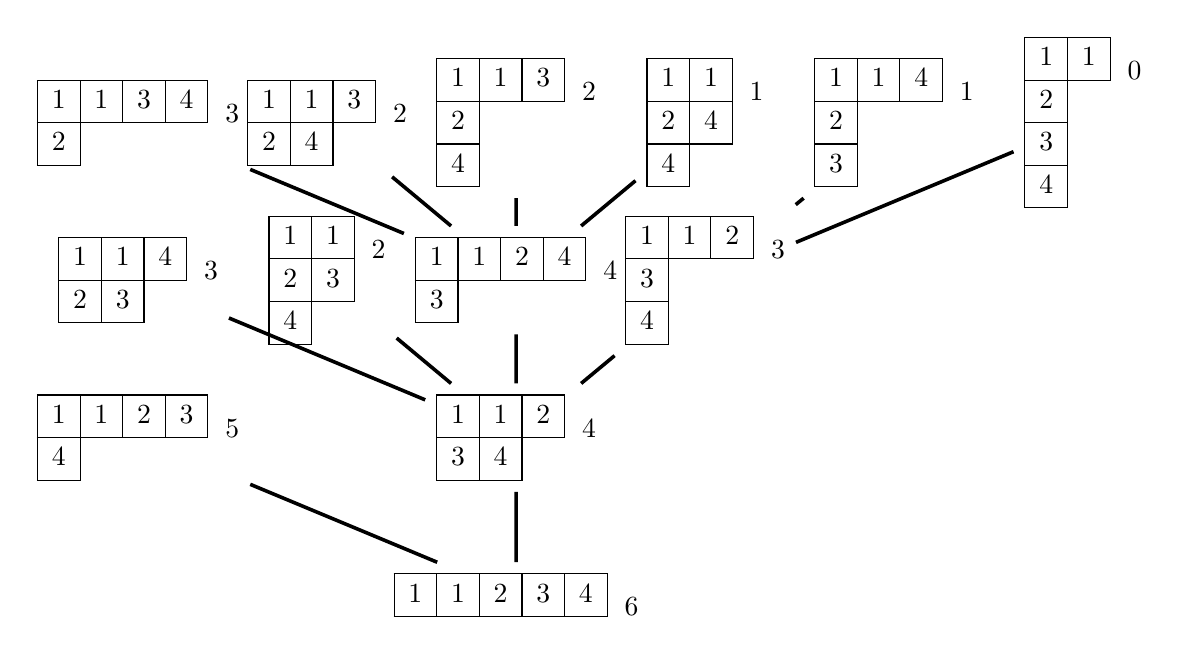
\begin{tikzpicture}[xscale=1.2, yscale=1.0,line width=1.3pt]

\node (R4N1) at (0, 6) {\ytableaushort{1134,2}\; 3};
\node (R4N2) at (2, 6) {\ytableaushort{113,24}\; 2};
\node (R4N3) at (4, 6) {\ytableaushort{113,2,4}\; 2};
\node (R4N4) at (6, 6) {\ytableaushort{11,24,4}\; 1};
\node (R4N5) at (8, 6) {\ytableaushort{114,2,3}\; 1};
\node (R4N6) at (10,6) {\ytableaushort{11,2,3,4}\; 0};

\node (R3N1) at (0, 4) {\ytableaushort{114,23}\; 3};
\node (R3N2) at (2, 4) {\ytableaushort{11,23,4}\; 2};
\node (R3N3) at (4, 4) {\ytableaushort{1124,3}\; 4};
\node (R3N4) at (6, 4) {\ytableaushort{112,3,4}\; 3};

\node (R2N1) at (0, 2) {\ytableaushort{1123,4}\; 5};
\node (R2N2) at (4, 2) {\ytableaushort{112,34}\; 4};


\node (R1N1) at (4, 0) {\ytableaushort{11234}\; 6};

\draw (R4N1) -- (R3N3);
\draw (R4N2) -- (R3N3);
\draw (R4N3) -- (R3N3);
\draw (R4N4) -- (R3N3);
\draw (R4N5) -- (R3N4);
\draw (R4N6) -- (R3N4);

\draw (R3N1) -- (R2N2);
\draw (R3N2) -- (R2N2);
\draw (R3N3) -- (R2N2);

\draw (R3N4) -- (R2N2);

\draw (R2N1) -- (R1N1);
\draw (R2N2) -- (R1N1);



\end{tikzpicture}




\end{document}
